\chapter{Testing and Analysis}
\label{testing}

This section of the report outlines the testing necessary in order to evaluate the accuracy and robustness of the volume reconstruction, volume and limb circumference calculation and the recording and recall of medical scanner postioning on the human body. This testing informs our evaluation of the project. It is the intention of the group to demonstrate that this non-invasive and 'hands-free' Kinect based methodology provides at least a good approximation of measurements achieved through more accurate means of testing. 

\section{Test Plan}

We prepared a test plan at the start of the project which acted as motivation for defining the internal deliverable deadlines. Along with this test plan, we have outlined a strategy by which to test each component of the system thoroughly.

\subsection{Test Strategy}

\label{test strategy}

Each functional aspect of the system has been unit tested by their respective group member with their results and analysis presented in each section of this chapter. The unit tests are concerned with the operation of: \emph{\bf{person isolation, registration, volume calculation, limb circumference, image recognition and database functionality.}} Integration testing is then performed and the functionality of respective modules tested against one another, for example, the scanning of patients being used along side the database engine and visualisation module. System-wide testing is then examined with a number of test cases that aim to evaluate the toolkit as one coherent system.

\subsection{Test Controls}

The environment in which subjects are to be captured must be as consistent as possible. As such the group have defined a number of controls that is imposed upon persons being scanned that will return the results with reasonable consistency and accuracy.\\

\emph{\bf{Distance from Kinect}} - In order to capture the entire body and to ensure consistent positioning between volume scans, the subject will stand at approximately 2.2m away from the Kinect. This distance was chosen, despite the fact it is outside of the Kinect's \emph{recommend play space} \cite{xbox2010}, as it is far enough away to accommodate subjects who are at the upper bound of test patients in terms of height without compromising too much on the quality of the captured depth map associated with the subject. Our configuration means that for each side of the patient that is scanned, this distance is maintained. The reconstruction process then does not need to take into account global scaling of the point cloud when translating and rotating it into position. \\

\emph{\bf{Position of the Kinect}} - In order to ensure fair test conditions, when a volume scan is taken the Kinect must be positioned 71cm off the floor. The scanning process will automatically change the elevation of the Kinect to 0 when a new scan is initiated.\\

\emph{\bf{Lighting Conditions}} - Scans were taken in the same environment where lighting was adequate but not too bright so as to interfere with the CMOS sensor's ability to track different levels of depth in the scene. Lighting was also important for the purposes of skeletal tracking as the SDK's algorithms relied on tracking the human body in RGB space for this purpose. \\

\emph{\bf{Occlusion and Noise}} - During development we found that the Kinect was particularily sensitive to noise leading to distorted depth maps where lighting was in adequate or there were objects in the foreground of the subject to be scanned. Occlusion was also an issue if the background was particularly crowded. We aimed to minimise the amount of noise and foreground interference by removing objects in the scene that may have otherwise interfered with the scan process. \\

\emph{\bf{Scan Process}} - The scan process itself is controlled by how it has been implemented. The subject is given 10 seconds to position themselves between each capture and by maintaining the ideal depth; a reasonably accurate scan can be captured permitting other influencing factors. \\

\emph{\bf{Clothing}} - Clothing presents an issue where the volume measurement or limb circumference measurement may be overly affected by a subject that is wearing baggy clothes or clothes that enlarge certain areas of the body. This has been identified as problematic in other 3D body scanning applications where the presence of clothing has interfered with the landmarking of particular areas of the body \cite{Dekker1999}. For the purposes of scanning we have requested that each subject remove any clothing apart from T-shirts and trousers in order to gain more accurate volume measurements and minimise subject discomfort. \\

\subsection{Test Schedule}

A test schedule was devised so that adequate testing of the volume estimation, limb circumference and marker-less tracking components of the system could be performed and changes made to them in order to ensure correct working functionality and accuracy when the system is eventually delivered to the customer. 

\begin{figure}
\centering
\begin{tabular}[htb]{| l | l | l |}
    \hline
    Unit Test & Date Started & Date Completed \\ \hline \hline
    Volume Estimation & 23/02/13 & 01/04/13 \\ \hline
    Limb Circumference & 25/03/13 & 23/04/13 \\ \hline
    Markerless Recognition & 01/04/13 & 20/04/13 \\ \hline
    Database Integration & 04/04/13 & 21/04/13 \\ \hline
    Unit Integration & 01/03/13 & 20/04/13 \\ \hline
    System Functionality & 05/04/13 & 21/04/13 \\ \hline
\end{tabular}

\caption{Test plan for the PARSE System}
\end{figure}


\section{Person Isolation}
\label{testing:person isolation}
This section details the testing of the depth based person isolation.\\

\subsection{Isolating Multiple Subjects}
During the design of depth based person isolation in Section \ref{imp:depth based isolation}, the isolation was determined to be sufficient for one person. Further testing was conducted on multiple subjects to confirm that the method would work on many people, rather than only the subject in Figure \ref{fig:depth and hand based cut off}. Figure \ref{fig:multiple subjects isolated} show the behaviour of the isolation method on the aforementioned multiple subjects. From this figure, the isolation method can be said to work consistently on many subjects.\\

\begin{figure}[h]
\begin{center}
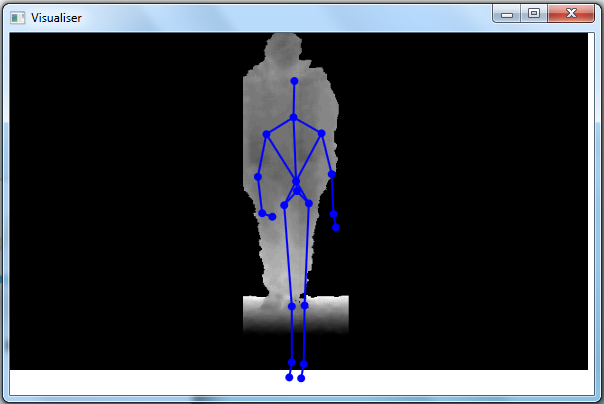
\includegraphics[scale=0.3]{images/bernie_iso} 
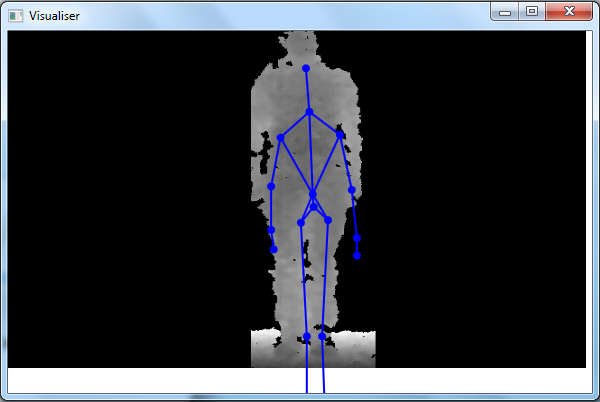
\includegraphics[scale=0.3]{images/page} 
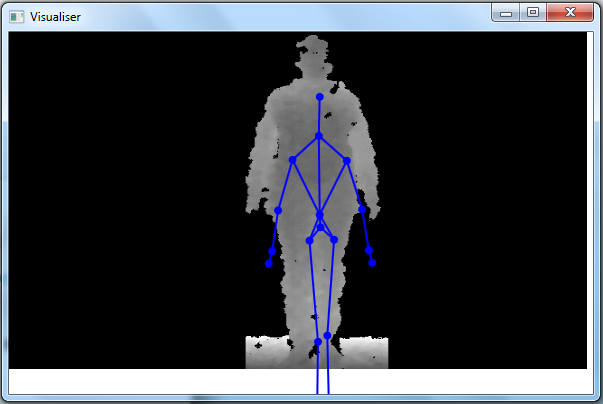
\includegraphics[scale=0.3]{images/steffat} 
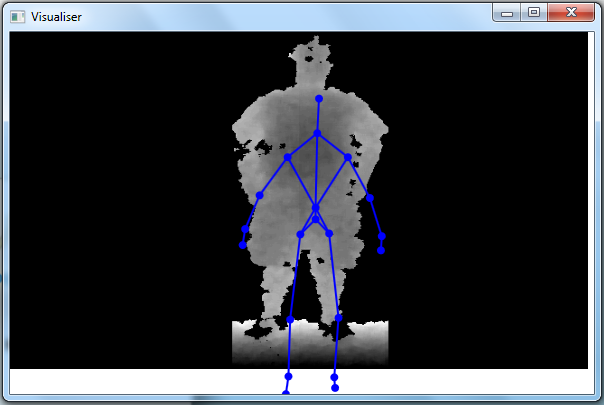
\includegraphics[scale=0.3]{images/wilkoiso} 
\end{center}
\caption{Multiple subjects isolated.}
\label{fig:multiple subjects isolated}
\end{figure} 

\subsection{Floor Removal}
As previous noted in Sections \ref{design:depth based isolation} and \ref{imp:depth based isolation}, the depth based cut off leaves the floor underneath the person as an unwanted artifact in the final point cloud. Fortunately, the floor can be removed at the point cloud level as suspected. An example of this action is shown in Figure \ref{fig:floor removal}.\\

\begin{figure}[h]
\begin{center}
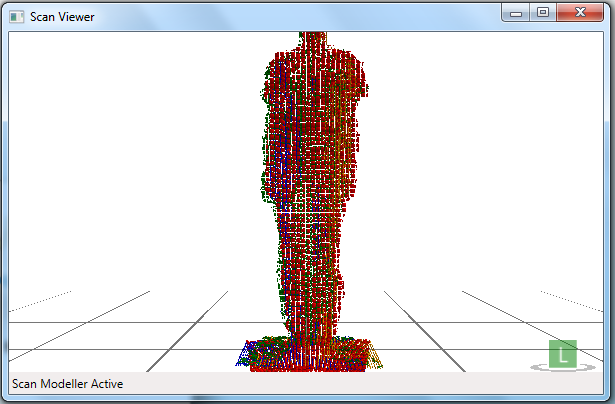
\includegraphics[scale=0.3]{images/greg_feet}
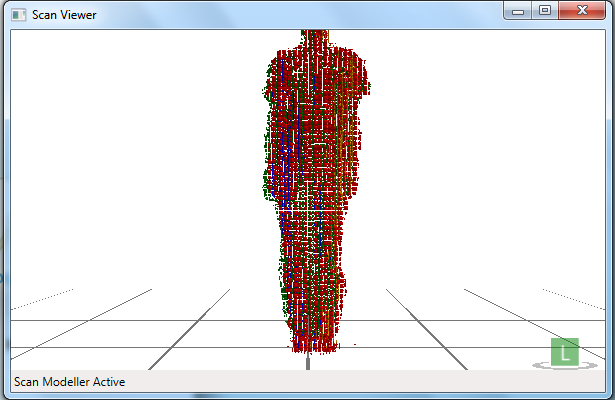
\includegraphics[scale=0.3]{images/greg_nofeet} 
\end{center}
\caption{Left: The point cloud with the floor. Right: After floor removal.}
\label{fig:floor removal}
\end{figure} 
\section{Registration}
\label{testing:registration}
This section deals with the testing of the registration functionality, as described in Section \ref{design:registration}. 

\subsection{Methodology}
Testing this sub-system was not a trivial exercise due to the interdependence with volume estimation. That is, correct volume estimation requires correct registration but the correctness of registration can only be measured by observing correct values of volume estimation.\\

The best way of determining the accuracy of stitching is by analying the deviance of the Toolkit Volume Measurement from the Gold Standard Volume measurement, which can be read in Section \ref{testing:vol est}. The first data point, Bernard, is a control and the error is irrelevant. \\
\section{Volume Estimation}
This section details the implementation of the chosen, SSP based volume estimation algorithm discussed in Section \ref{design:planimetry}. During this phase, several issues were overcome. \\

\subsection{How Many Planes?}
There was a necessary trade off between number of planes and quality of those planes. If the number of planes was too low, the volume estimation would be woefully inaccurate due to a lack of required granularity. If the number of planes was too high, then the volume would be inaccurate due to the lack of information contained within a plane. Sixty planes were chosen, based on a visual inspection of planes within the Corbett data set, shown in Figure \ref{fig:the_corbett_data_set}.\\

\begin{figure}[htb]
\begin{center}
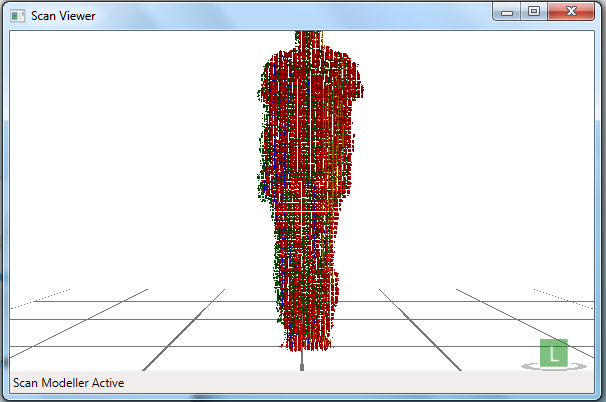
\includegraphics[scale=0.4]{images/corbett_dataset} 
\end{center}
\caption{The Corbett data set, stitched perfectly by the Bounding Box method}
\label{fig:the_corbett_data_set}
\end{figure}

\subsection{Noisy Data}
The data retrieved from the point clouds was not as originally expected. Firstly, the y-values were not discrete but continuous, as a result retrieving a plane at a single height would not result in ring of points. Therefore, a plane would be retrieved from a range of heights and then the points flattened to form a ring.\\

Also, the points were not close to a convex hull as expected, see Figure \ref{slice 30 from the corbett data set}, but were in fact quite noisy. As such, the points were \emph{sub-sampled} and then averaged to reduce noise. Sub-sampling by a factor of $n$ involved discarding $n-1$ points out of every $n$. Averaging points by a factor of $n$ involved adding the co-ordinate values of $n$ points, averaging them into a single point and returning a list of such average points. Figure \ref{plane 30 from the corbett data set sub-sampled and averaged} shows plane 30 of the Corbett data set after being sub-sampled and averaged by a factor of 7. A factor of 7 was chosen again based on visual inspection of the planes.\\

\begin{figure}[htb]
\begin{center}
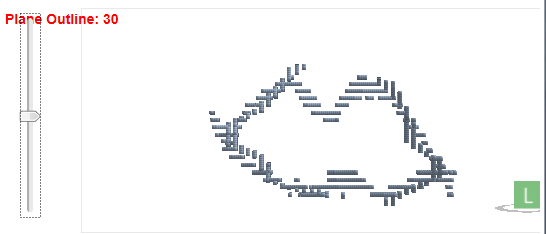
\includegraphics[scale=0.4]{images/notasexpected} 
\end{center}
\caption{Plane 30 from the Corbett data set}
\label{slice 30 from the corbett data set}
\end{figure} \\

\begin{figure}[htb]
\begin{center}
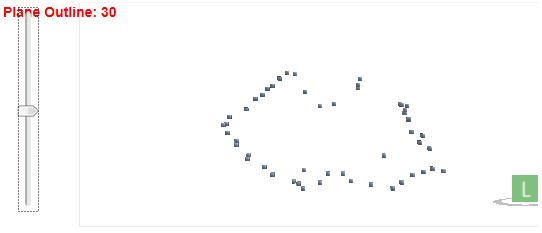
\includegraphics[scale=0.4]{images/improved} 
\end{center}
\caption{Plane 30 from the Corbett data set sub-sampled and averaged}
\label{plane 30 from the corbett data set sub-sampled and averaged}
\end{figure} \\

\subsection{The Need for a Transform Constant}
Early metrics returned were calculated in \emph{point cloud space} (PCS), as evidenced by the Corbett data subject's height being predicted as 2.27m. Therefore, a transform constant is required to move between measurements calculated in point cloud space (PCS) and measurements in terms of SI units in \emph{real world space} (RWS). Such a transform was believed necessary because the Kinect stores distances in terms of pixels and points, rather than meters and it is real world measurements that the calculated volume should be given. The transform was suspected to be multiplicative and as such is of the form shown in equation \ref{imp: transform between pcs and rws}. Determination of this constant was determined empirically during testing.\\

\begin{equation}
Volume_{PCS} * Transform Constant = Volume_{RWS}
\label{imp: transform between pcs and rws}
\end{equation}\\
\section{Limb Circumference}
\label{testing:limb circumference}
This section details the testing of the limb circumference algorithms. Circumference testing in the context of volume estimation is discussed and the equivalent accuracy of partitioned plane circumference estimation examined to validate whether such practice produces a reliable means for estimating limb size.

\subsection{Calculating Limb Bounds}

The 20 feature points provided by the skeleton are used to simplify the bounding of by referencing the minimal and maximal feature points of the interested limb. An assumption is made that the detected skeletal positions are reasonably aligned with the respective limb locations captured by the point cloud. \\

\begin{table}[!htb]
\begin{center}
  \begin{tabular}{| l | p{4cm} | r | r | r | r |}
    \hline
    Limb & Feature Points & $X_{min}$ & $X_{max}$ & $Y_{min}$ & $Y_{max}$ \\ \hline 
    Left Arm & ShoulderLeft, WristLeft & 0.250 & 0.267 & 0.0779 & 0.778  \\ \hline
    Right Arm & ShoulderRight, WristRight & -0.191 & -0.1652 & 0.03 & 0.808  \\ \hline
    Shoulders & ShoulderRight, ShoulderLeft & -0.61 & 0.251 & 0.462 & 0.947 \\ \hline
    Waist & HipRight, HipLeft, HipCenter & -0.053 & 0.138 & 0.270 & 0.371  \\ \hline
    Right Leg & HipCenter, HipRight, KneeRight, FootRight & -0.051 & 0.040 & -0.523 & 0.280  \\ \hline
    Left Leg & HipCenter, HipLeft, KneeLeft, FootLeft & 0.045 & 0.131 & -0.519 & 0.270  \\ \hline
  \end{tabular}
\end{center}
\caption{Feature points for each limb as recorded by Corbett Subject}
\label{testing: feature points used for each limb}
\end{table}

These limbs bounds are determined based on the anatomical reference points that the Kinect Skeleton SDK attaches to the tracked skeleton when undergoing a scanning procedure. The bounding is identified when the person is facing the front as the SDK is only capable of inferring skeletal cues when the subject is in a frontal configuration. The depth of the subject is defined in terms of the stitched point cloud where the minimum depth is recorded at the front and the maximal depth offset against the rear scan.

\subsection{Identifying Transform Constants}

As discussed in Section \ref{volume estimation}, there is a need for identifying transform constants between the circumferences calculated in terms of point cloud units and real-world and meaningful SI units. Using the height transform constant for the purposes of scaling circumference still provides a valid basis for accurate limb measurement as there is a broadly positive correlation between the height of an individual and in the cited cases, their arm circumference \cite{Todorovic2003}. However, on a local limb circumference measurement level, factors such as clothing, point cloud quality and the stability during of the person during scanning influences the integrity and accuracy of the planes extracted from the partitioned point clouds. \\

After bounding the limbs, the circumference of the subsampled planes is calculated. This circumference value represents the circumference with respect to the point cloud coordinate system and even when converted to standard units, the value is comparably small due to the lack of associated scale associated with it. A number of experiments have been carried out on subjects in order to determine these scale factors across a fairly representative spread of size and shape. The transform constants have been established from a subsample of the original sample of test subjects and classified according to below average, average and above average weight and overall size. \emph{Below Average} is determined as below 60kg and/or less than 1.6m in height. \emph{Average} is determined as between 60kg and 90kg and/or between 1.6 and 1.9m in height. \emph{Above Average} is determined as over 90kg or over 1.9m in height.  $Rw$ refers to the raw circumference as determined from calculation in the point cloud space, $Ac$ refers to the circumference as defined by spring tape measurement with a constant calculated from the difference.

\begin{table}[!htb]
\begin{center}
\begin{tabular}{| l | l | l | l | l |}
\hline
Subject & Limb & $Circum_{Rw}$ & $Circum_{Ac}$ & Transform Constant \\ \hline
    Below Average & Left Arm & 21.341 & 25.8 & 1.21 \\ \hline
    & Right Arm & 22.34 & 23.4 & 1.05\\ \hline
    & Shoulders & 57.22 & 82 & 1.43\\ \hline
    & Chest & 49.3 & 80 & 1.62\\ \hline
    & Waist & 11.3 & 75 & 6.63\\ \hline
    & Left Leg & 9.2 & 35.6 & 3.89\\ \hline
    & Right Leg & 12.3 & 36.5 & 2.96\\ \hline \hline
    Average & Left Arm & 23.195 & 25 & 1.07 \\ \hline
    & Right Arm & 24.12 & 25.5 & 1.05 \\ \hline
    & Shoulders & 64.39 & 92 & 1.41\\ \hline
    & Chest & 61.19 & 91.5 & 1.42\\ \hline
    & Waist & 14.82 & 88 & 5.94\\ \hline
    & Left Leg & 13.05 & 40.5 & 3.10\\ \hline
    & Right Leg & 14.9 & 44.0 & 2.95\\ \hline \hline
    Above Average & Left Arm & 35.443 & 32.5 & 0.91\\ \hline
    & Right Arm & 34.53 & 31 & 0.89\\ \hline
    & Shoulders & 68.123 & 104.5 & 1.53\\ \hline
    & Chest & 67.980 & 99.5 & 1.46\\ \hline
    & Waist & 22.3 & 101 & 4.529\\ \hline
    & Left Leg & 16.501 & 56 & 3.39\\ \hline
    & Right Leg & 16.091 & 56.5 & 3.51 \\ \hline \hline
\end{tabular}
\end{center}
\caption{Transform constants calculated for the required correction of different subject circumferences based on spring tape measurements.}
\label{testing: transform constants}
\end{table}

\subsection{Errors and Limb Circumference}

As shown in each person classification above, there is in some cases, a requirement for significant correction of the the recorded point cloud circumference when compared to the circumferences recorded using spring tape measurement. The need for this correction is particularly profound around the lower extremities of the body with the worst case being recorded in the lower than average person on the waist necessitating a 6.5 scaling factor to align the toolkit's measurement with what is realistically expected. Through further testing it was ascertained that the patient scanning configuration where the legs were positioned close together was not an optimal configuration for mapping the skeletal co-ordinates into point cloud space. This was due to the Kinect API's inability to infer both the left and right legs properly and inferring the waist from the straight arm configuration in the upper extremities. In some cases this lead to a deviation of $[-0.5,0.5]$ from the original assumed centre of the limb in point cloud space from the inaccurate recording of limb positioning from the Kinect SDK. \\

Obviously further refinements were needed to the point cloud partitioning bearing in mind the sometimes erroneous or imprecise mapping of the skeletal world coordinates to point cloud space. When refinements were added so that tighter bounds were specified over particular limbs, a marked improvement was seen in the circumference calculation of upper extremities such that an average error of $10\%/15\%$ was observed. There was also an improvement on waist measurements due to the incorrect bounding method that was originally applied. Given these refinements, an average error over upper extremities (in the present results, the left arm) ranged between $2.0\% - 17\%$ and lower extremities varied between $10\%-36.6\%$. \\

\begin{table}[!htb]
\begin{center}
  \begin{tabular}{| l | r | r | r | r | r | r |}
    \hline
    Person & $Arm_{Ac}$ & $Waist_{Ac}$ & $Arm_{Ki}$ & $Waist_{Ki}$ & $Error_{arm}$ & $Error_{waist}$  \\ \hline
    Corbett & 27 & 84 & 25.9 & 69.33 & 4.2\% & 21.1\% \\ \hline
    Eddie & 27.2 & 81.9 & 23.1 & 59.3 & 17\% & 36\% \\ \hline
    Page & 24.5 & 82 & 24 & 72 & 2.01\% & 13.8\% \\ \hline
    Papas & 23.5 & 89 & 26.13 & 65.13 & 11.1\% & 36.6\% \\ \hline
    Rodolis & 25 & 91 & 29 & 73.4 & 16\% & 23.9\% \\ \hline
    Sexton & 26.4 & 83 & 24.80 & 72.1 & 6.5\% & 15.1\%\\ \hline
  \end{tabular}
\end{center}
\caption{Errors measured over 6 test subjects.}
\label{testing: table of data for limb transform constants}
\end{table}

\subsection{Sources of error}

There are a number of potential error sources that result in the error observed in these results and some have already been alluded to. There are 3 primary areas where error is introduced into the limb circumference calculation:

\begin{enumerate}
    \item \emph{Poor point cloud registration}; where the stitching algorithms for registering each of the 4 point cloud scans returned poor results, the circumference measurements were affected by the lack of the required ring of points needed for circumference calculation so the gift wrapping algorithm would often calculate the circumference for a subset of possible points returning results that were infeasibly small as a result.
    \item \emph{Clothing}; normal clothing or baggy items of clothing often obscure the true value of the circumference, especially around the waist, leg and arm areas. It is likely that in the case of some subjects that their circumferences were over-estimated due to the amount of clothing that may have been present in some areas of the body during scanning.
    \item \emph{Noise and Sensor Distance}; the amount of noise present in the Kinect meant that our Point Cloud combined with the sensor distance from the subject was of a low resolution and this meant that the gift wrapping algorithm sometimes calculated the circumference around a ring of points selectively or overestimated where there were outliers in the plane.
    
\end{enumerate}

\subsection{Monitoring Limb Changes}

The ongoing monitoring of limb circumference based on this method is considered reasonably accurate for cases where the variation in the circumference is sufficient enough to highlight a difference between it and a previous circumference scan over a period of time. Local changes in the limb such as body fat distribution in particular areas of interest such as the upper arm where the study of the distribution of body fat and skin folds in this area can reveal information about medical conditions or ongoing weight gain/loss from a particular treatment program are harder to identify using this method. This is due to the limitations already outlined with the noise and low resolution of the depth map at local levels of the point cloud unless the limb is of sufficient size.

\pagebreak
\section{Markerless Recognition}
Several tests were conducted, to assess the performance of the proposed solutions to the tracking and registration problems.\\

\subsection{Colour Search}
The testing phase for the colour scanner began with the RGB colour space. Being the simplest to work with, as the imagery is output in ABGR format (simply RGBA in reverse order), the results were obtained very quickly.\\

\subsubsection{Results}
Searching for colours in the RGB colour space was quite effective, but key factors influenced results negatively.\\

Firstly, lighting affects the reflected colour of an object greatly, and is difficult to account for. In uneven or directed lighting most objects will have gradients across them due to the combination of their shape with the direction of the predominant lighting. This means that when searching for the exact colour of an object, the result gives typically very few pixels on the object matching exactly that colour. Here, by ‘exact colour’ we mean the colour of a selected pixel from the object image. \\

This is the key drawback of the RGB colour space for this type of search, which, theoretically, the HSL colour space could help avoid.\\
Allowing for a range of colours, defined by allowing a specified variance above and below the target colour component values, helps to account for the variation in colour and shade on an object.\\

\subsubsection{Choosing Colours}
Dark colours are poor for tracking. One cause in particular is that dark areas are highly susceptible to noise, which is a key burden of working with low-cost hardware. Dark areas rarely contain the target colour in great quantities, rather a miscellany of colour produced by the sensor. Interestingly, this also causes issues when searching for mid-brightness colours; dark regions occasionally cause flecks of brighter colour which may be in the search range.\\

Brighter colours, therefore, are better for this application. Still, a problem remains in deducing which colour is best for tracking in the target environment. Approaching pragmatically, reds are highly present in photography of people, being a strong component in the colour of skin; and is often a primary indicator of skin in image analysis. Red tones are also prominent in wood, thus appearing regularly in many furnishings. Blue is a prominent colour in NHS equipment, clothing, signage and so forth. Green, however, although ubiquitous in natural scenes, is rarely found in office or medical scenes. Certainly in our testing environment, there were very few green objects.\\

To confirm this, we took a pack of brightly coloured papers and attempted to track them. The pack provided paper in green, yellow, orange and pink. For each colour, we tried using a click-to-match function in our micro-application to see if the paper would be tracked at all, and then assess its visibility at 2.2m distance.\\

\begin{table}
\centering
  \begin{tabular}{| r | r | r | r | r |}
    \hline
    Variance & Green & Orange & Pink & Yellow \\ \hline
    0 & 2 & 4 & 5 & 10\\ \hline
    10 & 1500 & 900 & 1100 & 1300\\ \hline
    20 & \textit{2700} & \textit{2000} & \textit{1900} & \textit{2300}\\ \hline
    30 & \textbf{3300} & 2900 & \textbf{2800} & 2700\\ \hline
    40 & 3900 & 4200 & 9000 & \textbf{3600}\\ \hline
    50 & 4900 & \textbf{7000} & 28000 & 4300\\ \hline
    60 & 7900 & 9800 & 47000 & 5000\\ \hline
  \end{tabular}
    \caption{Filter responses to different colour targets with increasing variance. Italics indicate when the shape was fully and evenly shown. Bold indicates the point at which the target center was most accurately found.}
\end{table}


\subsubsection{HSL Colour Space}
The HSL colour space, by separating hue from shade, potentially allows far greater flexibility under different lighting conditions.
Testing the HSL colour space followed the test mantra laid out by the RGB space experiments. Attempting to track the same sheets of paper, it was found that our mechanism in fact made it harder to track. \\

\begin{table}
\centering
  \begin{tabular}{| r | r | r | r | r |}
    \hline
    Variance & Green & Orange & Pink & Yellow \\ \hline
    0 & 0 & 0 & 0 & 0 \\ \hline
    10 & 100 & 500 & 360 & 150 \\ \hline
    20 & \textit{1200} & 1200 & \textit{2300} & \textit{\textbf{1300}} \\ \hline
    30 & \textbf{1900} & \textit{\textbf{1800}} & 4100 & 2400 \\ \hline
    40 & 3900 & 2200 & 7250 & 3900 \\ \hline
    50 & 4500 & 3100 & 13900 & 5871 \\ \hline
    60 & 5300 & 4600 & 59000 & 7700 \\ \hline
  \end{tabular}
    \caption{Filter responses to different colour targets with increasing variance. Italics indicate when the shape was fully and evenly shown. Bold indicates the point at which the target center was most accurately found.}
\end{table}

The results given by the HSL tracker differ greatly in appearance to those from the RGB tracker. Although a similar mechanism is in place, it appears as though the .HSL tracker is more specific; as the variance is increased, the additional pixels shown are not in contiguous clumps as with the RGB tracker. Rather, the new pixels appear sporadically around the image. This could allow better opportunities for noise removal, as the individual pixels can be cancelled out a lot more easily than blocks.\\

\begin{figure}
\centering
  \begin{tabular}{ c }
    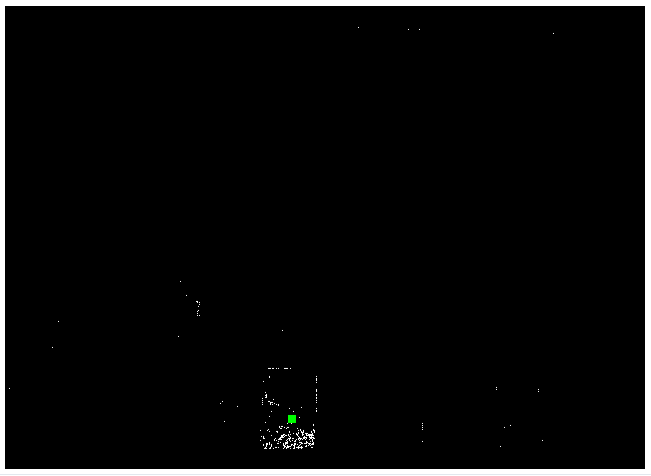
\includegraphics[scale=0.25]{zscreenshots/hsl_green_20}\\ 
    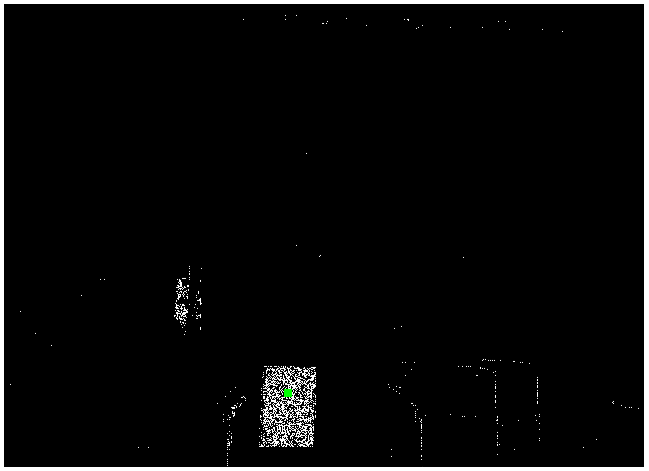
\includegraphics[scale=0.25]{zscreenshots/hsl_green_30}\\ 
    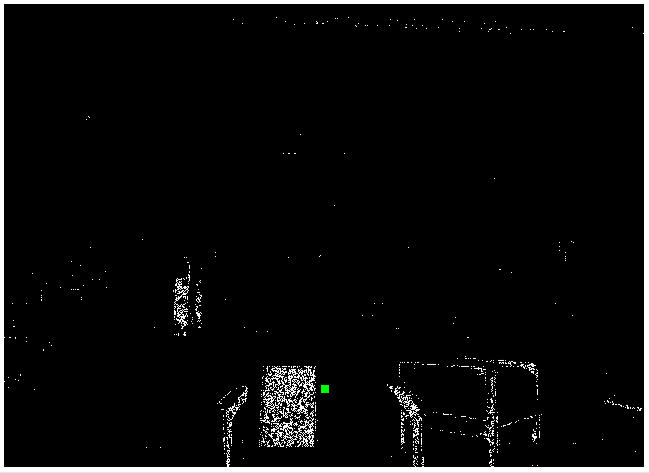
\includegraphics[scale=0.25]{zscreenshots/hsl_green_40}\\ 
    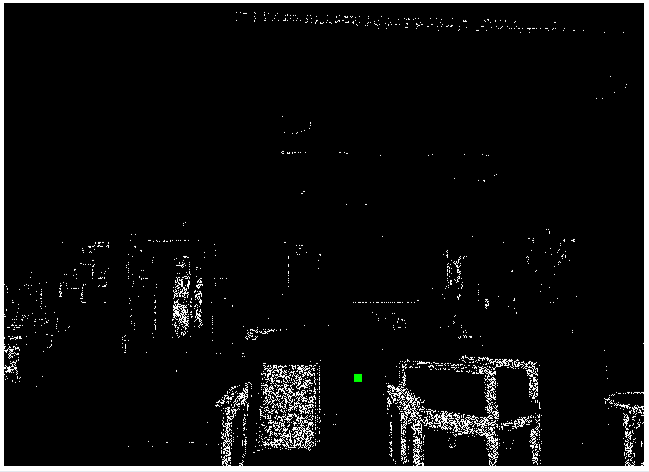
\includegraphics[scale=0.25]{zscreenshots/hsl_green_60}\\ 
    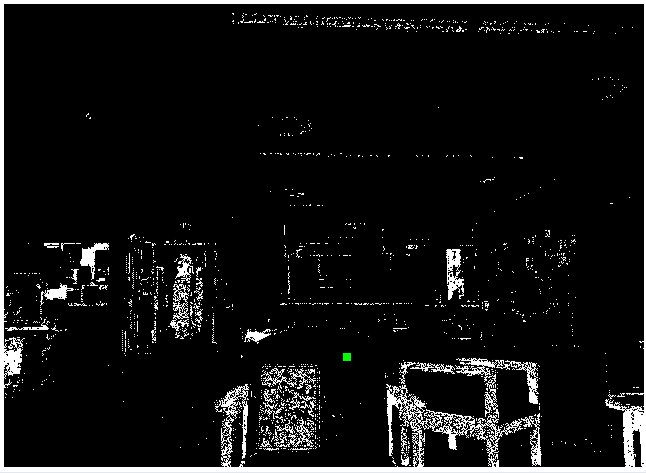
\includegraphics[scale=0.25]{zscreenshots/hsl_green_80}\\
  \end{tabular}
    \caption{Increasing the variance begins to allow colours from the environment.}
\end{figure}

Above 2000 found pixels, the added pixels from variance increase were from the environment more than from the paper. As such, the pink paper never gave a useful result for tracking. A major contributor to this was the slight pinkish hue of the paintwork – never particularly noticed until these tests – which came into range as the increased variance allowed for more subtle colours.\\


\subsubsection{Summary}
Despite key obstacles, tracking in the RGB space worked surprisingly well. Based on a simple, almost primitive, idea, it outperformed the, more complex, HSL colour space search quite competitively. Not only that, but it was much faster to compute. The average frame took 300ms with the RGB search, and 700ms for HSL: a significant difference for a system aiming to provide results in real time.\\

\subsubsection{Lighting}
Lighting, as can be expected, did cause issues. The testing area is subject to strong side lighting from the windows, which causes the angle of the paper to affect perceived colour dramatically. This increased the importance of being able to search for a colour range, rather than a specific colour only.\\

An interesting factor that had an effect on the results was the exposure of the imagery. The exposure time seems to quite drastically affect the colours given – especially for the HSL format imagery, which accounts for lightness and saturation – which reduces the effectiveness of the mechanism. Being beyond our control, it adds a layer of complexity to the HSL imagery which would be very hard to account for.\\

Received light at the sensor is not only affected by the light sources, but the reflecting materials in view. The paper in use, being in texture matte rather than shiny, performed better than some other objects tested, which accentuated the specular lighting. There exist materials with ideal optical properties that would reduce such strong lighting effects further, but this begins to run beyond the scope of the project. Nonetheless, the use of a specific material coating on the sensor could be considered an acceptable modification to allow use of the system, and is worth mention.\\


\subsection{Haar}
The generation of the Haar classifier was to be fraught with complex procedures and intricate setup details. It took several weeks’ research and development to train a classifier at all, before testing could begin.\\

Limitations to this progress were numerous. For classifier use, the PCL library imports a classifier from a file, which is generated externally. To train the classifier, a precise setup must be created, and then generated through use of an executable via an obscure command line process. Further, the training process requires large numbers of training images. The documentation suggested minimal numbers in the order of thousands; a quantity which would take quite some time to collect.\\

The first experiment was, therefore, to find the minimum number of samples required to find a simple object. An application was created to allow the import, classification, and export of images into the correct formats and directory structures required for the training process. A sample of fifty positive, classified images and fifty negative images was found to be sufficient to generate a classifier.\\
Initially, a classifier was generated for a spectacles case – a simple object to hand with a featureful logo and interesting texture. The minimal classifier returned no result.\\
 
This test was important, because it raised important issues. First, would it be feasible to spend many more hours collecting sample data?  Secondly, was a Haar classifier a good choice to use at all? The answer, quickly realised, was no. The restrictions in effectiveness and in training and operation mean that for this application Haar classifiers simply aren’t powerful enough. For clear shapes and structures such as faces, they are well suited. But for this application numerous well-trained classifiers would be required to recognise just one object at various rotations. For the intended real-world application, several different sensors may need to be used and tracked, which raises the issue of training many different classifiers with many input images – too large a problem to be tackled.\\


\subsection{SURF}
The SURF classifier was tested on several different types of imagery to assess its performance. With the placement of synthetic features onto the sensor an allowable possibility, tests were devised to test SURF’s performance on both objects and on synthetic features in order to find a setup with sufficient performance.\\

The test suite included:
\begin{itemize}
\item Detection of objects in photographic imagery
\item Feature detection on synthetic features
\item Detection of synthetic features in synthetic imagery
\item Detection of synthetic features in photographic imagery
\end{itemize}
\\
Detection of objects in photographic imagery
Feature detection on synthetic features
Detection of synthetic features in synthetic imagery
Detection of synthetic features in photographic imagery
\\
\subsubsection{Natural Objects}
Images were taken at 2.2m using a digital camera, with a target object in view. Positive samples were taken of the target object at close range. These images were then run through the SURF classifier.
The testing on objects did not provide the positive results expected. Early testing indicated that, even at close range, what appears by eye to be a featureless object indeed has very few features identified.\\

\begin{figure}
\begin{center}
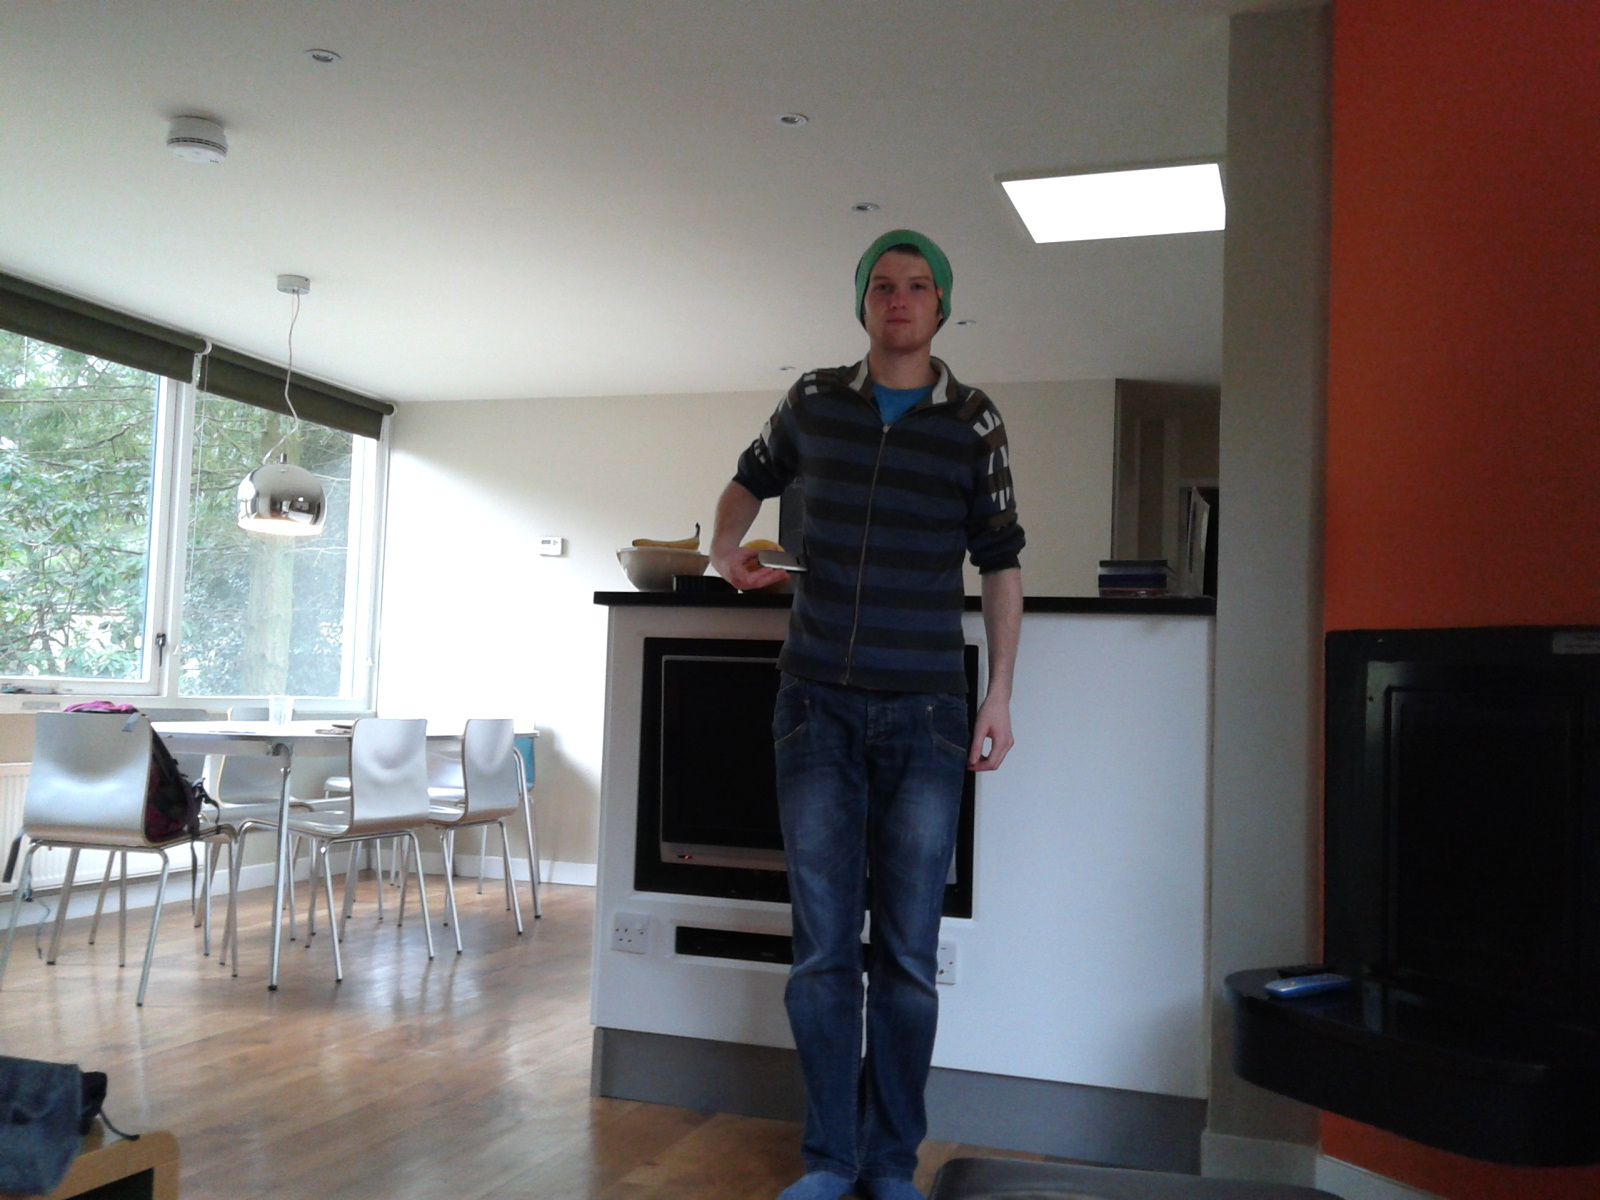
\includegraphics[scale=0.18]{images/20130207_134914.jpg}
\caption{Searching for the target object at distance}
\end{center}
\end{figure}

Part of this is due to SURF’s filtering of features: the initial feature detection will find several thousand features, which are then filtered to retain only those of particular ‘interest’. There is, therefore, no guarantee that the same features will be found in all situations.\\

\begin{figure}
\begin{center}
    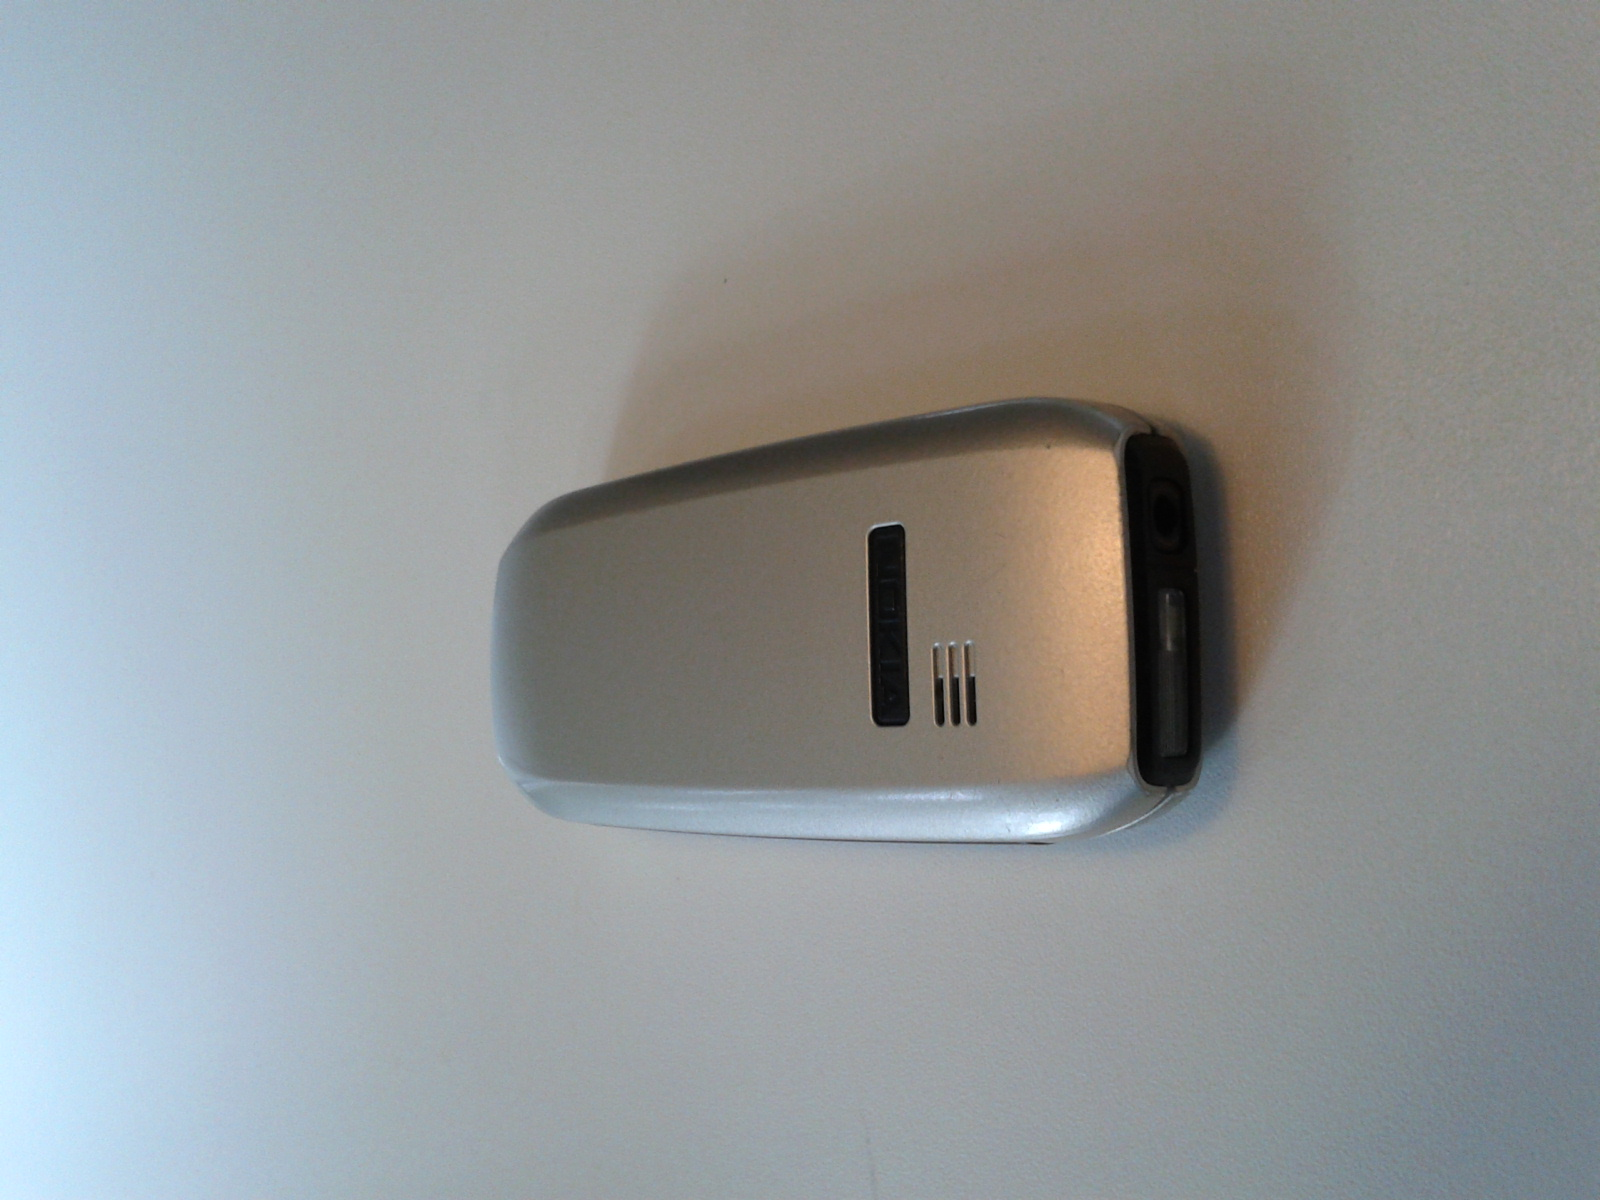
\includegraphics[scale=0.18]{images/20130207_134729.jpg}
    \caption{The target object}
\end{center}
\end{figure}

The target close-ups were cropped and cleaned in order to provide a totally featureless background, such that all features found in the images would be on the target. This is a standard practise. Of further note is the use of target imagery at close range, when the target in the field is at distance. The intention was to see whether this aided feature finding, but clearly it does not. For a high-powered system, it might be possible to have either a series of target images at varying distances, or some internal representation of the target that can be used to model it at any distance, but that is not that case.\\

\subsubsection{Synthetic Features}
Various academic papers and examples show SURF working well, but those examples are typically on carefully constrained example objects, and of course don’t show what SURF didn’t work well on. As it has been shown to work poorly on plain objects, the suggestion to devise some synthetic feature to place upon the target seems sensible. \\

\begin{figure}
\begin{center}
    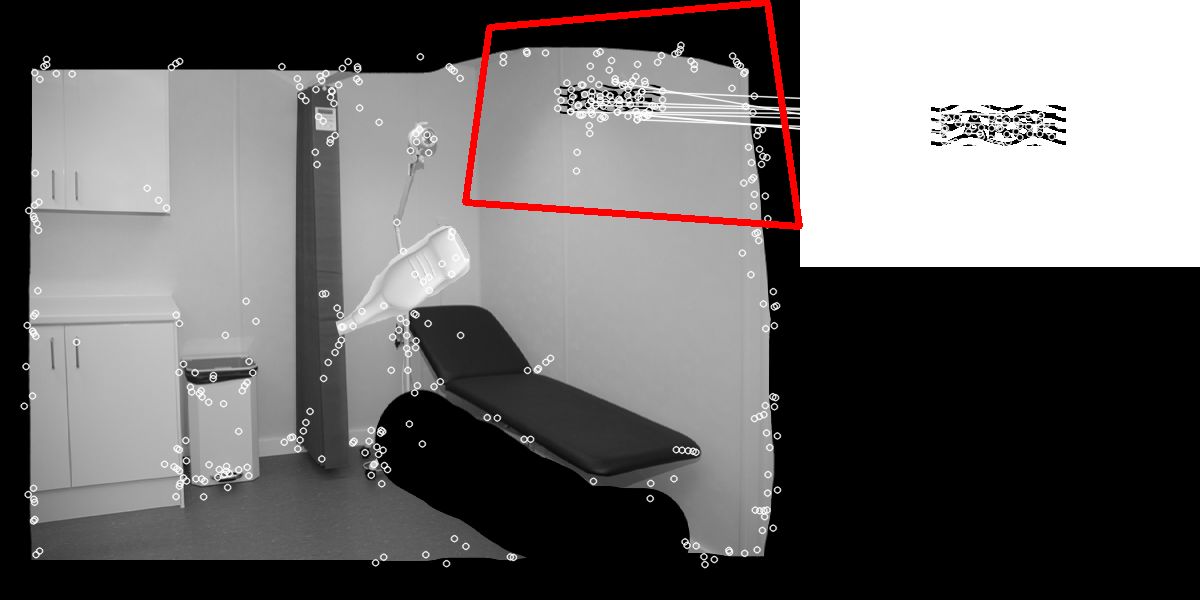
\includegraphics[scale=0.25]{images/synthetic_features_1.png}
    \caption{A synthetic feature inserted into an image, successfully found at near 1:1 scaling.}
\end{center}
\end{figure}

A collection of synthetic features of varying complexity was designed. Each feature was then rescaled in a second image, and the SURF detector used to search for the rescaled feature. The features designed contain different types of features known to be found by the SURF mechanism. \\

The previous problem of unreliable feature sets appeared again at the forefront – when rescaled, the detector found different sets of features. \\

\subsection{The Final Tracking Mechanism}
The system used to track the scanner was the RGB colour search, as it proved under testing to be the most reliable. That said, it was by no means completely reliable. The objects used, particularly under the highly directional lighting of the lab, were subject to specular lighting which reduced the surface area detected. This meant that in around 10\% of frames nothing was found at all. Also with random detected flecks around the room (including edges of plants visible through the glass panel in the door), the feed was quite difficult to work with in its raw form. A very simple mechanism was needed to steady the motion.\\

To perform this the median function was applied on a three frame window. This very effectively covered the holes and anomalies in the data, as neither zeros nor random high or low values would be the median value unless the sensor were detected there for more than one frame - in which case it is possible that the sensor has indeed moved. This made the feed much more stable, but still not completely so.\\

\subsection{Relocating Recorded Scan Positions}
Once stored in the database, recorded scan positions can be re-scanned. The project uses the previously described mechanisms to track the sensor's position relative to the body, except now on every frame. A distance metric is displayed to indicate how close the scanner is to the target position. Again, a capture mechanism is in place to allow the triggering of data capture from a real device.\\

\subsection{Conclusions}
The reliability of the tracking does limit the usability of the system. Overall, what should have been effective display from a set of modern algorithms was hampered by image quality and environmental issues.\\

The low resolution of the imagery, in combination with the environment and the operational properties of the SURF algorithm led to its poor result. As for the Haar classifier, it was quite possibly never going to work. It is difficult to assess how algorithms will perform, without a very full understanding of their operation. Such also are the difficulties of understanding how an algorithm will perform in different applications, scenarios and datasets, that often the best, and only, way to find out is to try.\\

Having made great effort to see a robust, feature-driven algorithm solve the problem, it is disappointing to find that our selections were ineffective, and that it is the almost trivial colour search in the RGB format that provided the only usable solution.\\

\subsection{Further development}
The RGB colour search was rightly the method chosen to drive the sensor tracking. Although lighting affects it so much, it is a fairly stable mechanism under consistent lighting, and is very easy to reconfigure if necessary; much unlike the ordeal required to train a new Haar classifier.\\

\subsubsection{Improving the tracking}
Part of the problem with the RGB tracking mechanism was that the whole environment was searched. One improvement, which was attempted as an aside but not completed, would be to use the depth data as a mask. Removing from the colour frame all regions behind the subjects would reduce drastically the noise present in the image, making tracking simpler whilst also more accurate.\\

The ability to control the lighting itself would be a highly desirable addition.\\



\newpage
\section{Summary}
This section summarises the testing undertaken.\\

\subsubsection{Person Isolation}
The person isolation has been shown to successfully isolate a variety of people and the floor can be isolated at a point cloud level.\\

\subsubsection{Volume Estimation}
An average transform constant has been calculated to be 0.81 (to two decimal places). The height estimation has an error of $\pm$4.25\% within the range tested and can repeatedly measure a subject to within $\pm$2\% on average.\\

The volume estimation could be said to have a minimum accuracy of between $\pm$1.06\% and $\pm$9.12\%. Whereas in practice the average error is 23.05\%, although this may be down to clothing and the relative ratios of subject volume is preserved to 0.62\%, but more test subjects are needed before any real conclusions can be made.\\

\subsubsection{Markerless Recognition}
Even with motion smoothing, the result from the RGB-based tracking mechanism is very shaky, and is strongly affected by lighting and the environment. Tracking is possible, but is not very reliable. The translation to real-world coordinates is largely accurate when the target tracking is stable, but only to +/- 2mm due to the resolution of the imagery.\\